% !TEX root = ../../semexp-thesis.tex

\section{Exploring Text Formatting through Semantic Conversations}
\label{sec:application/conversation}

In this scenario, we describe how a programmer uses a semantic conversation to explore Squeak's programming interface for creating formatted texts.
In Squeak, the \code{Text} class represents a formatted text that is modeled through a string and a run-length encoded array of nested sets of instances of a \code{TextAttribute} class hierarchy that provide different instructions to the text renderer.

\FloatBarrier
\begin{figure}[t]
	\centering
	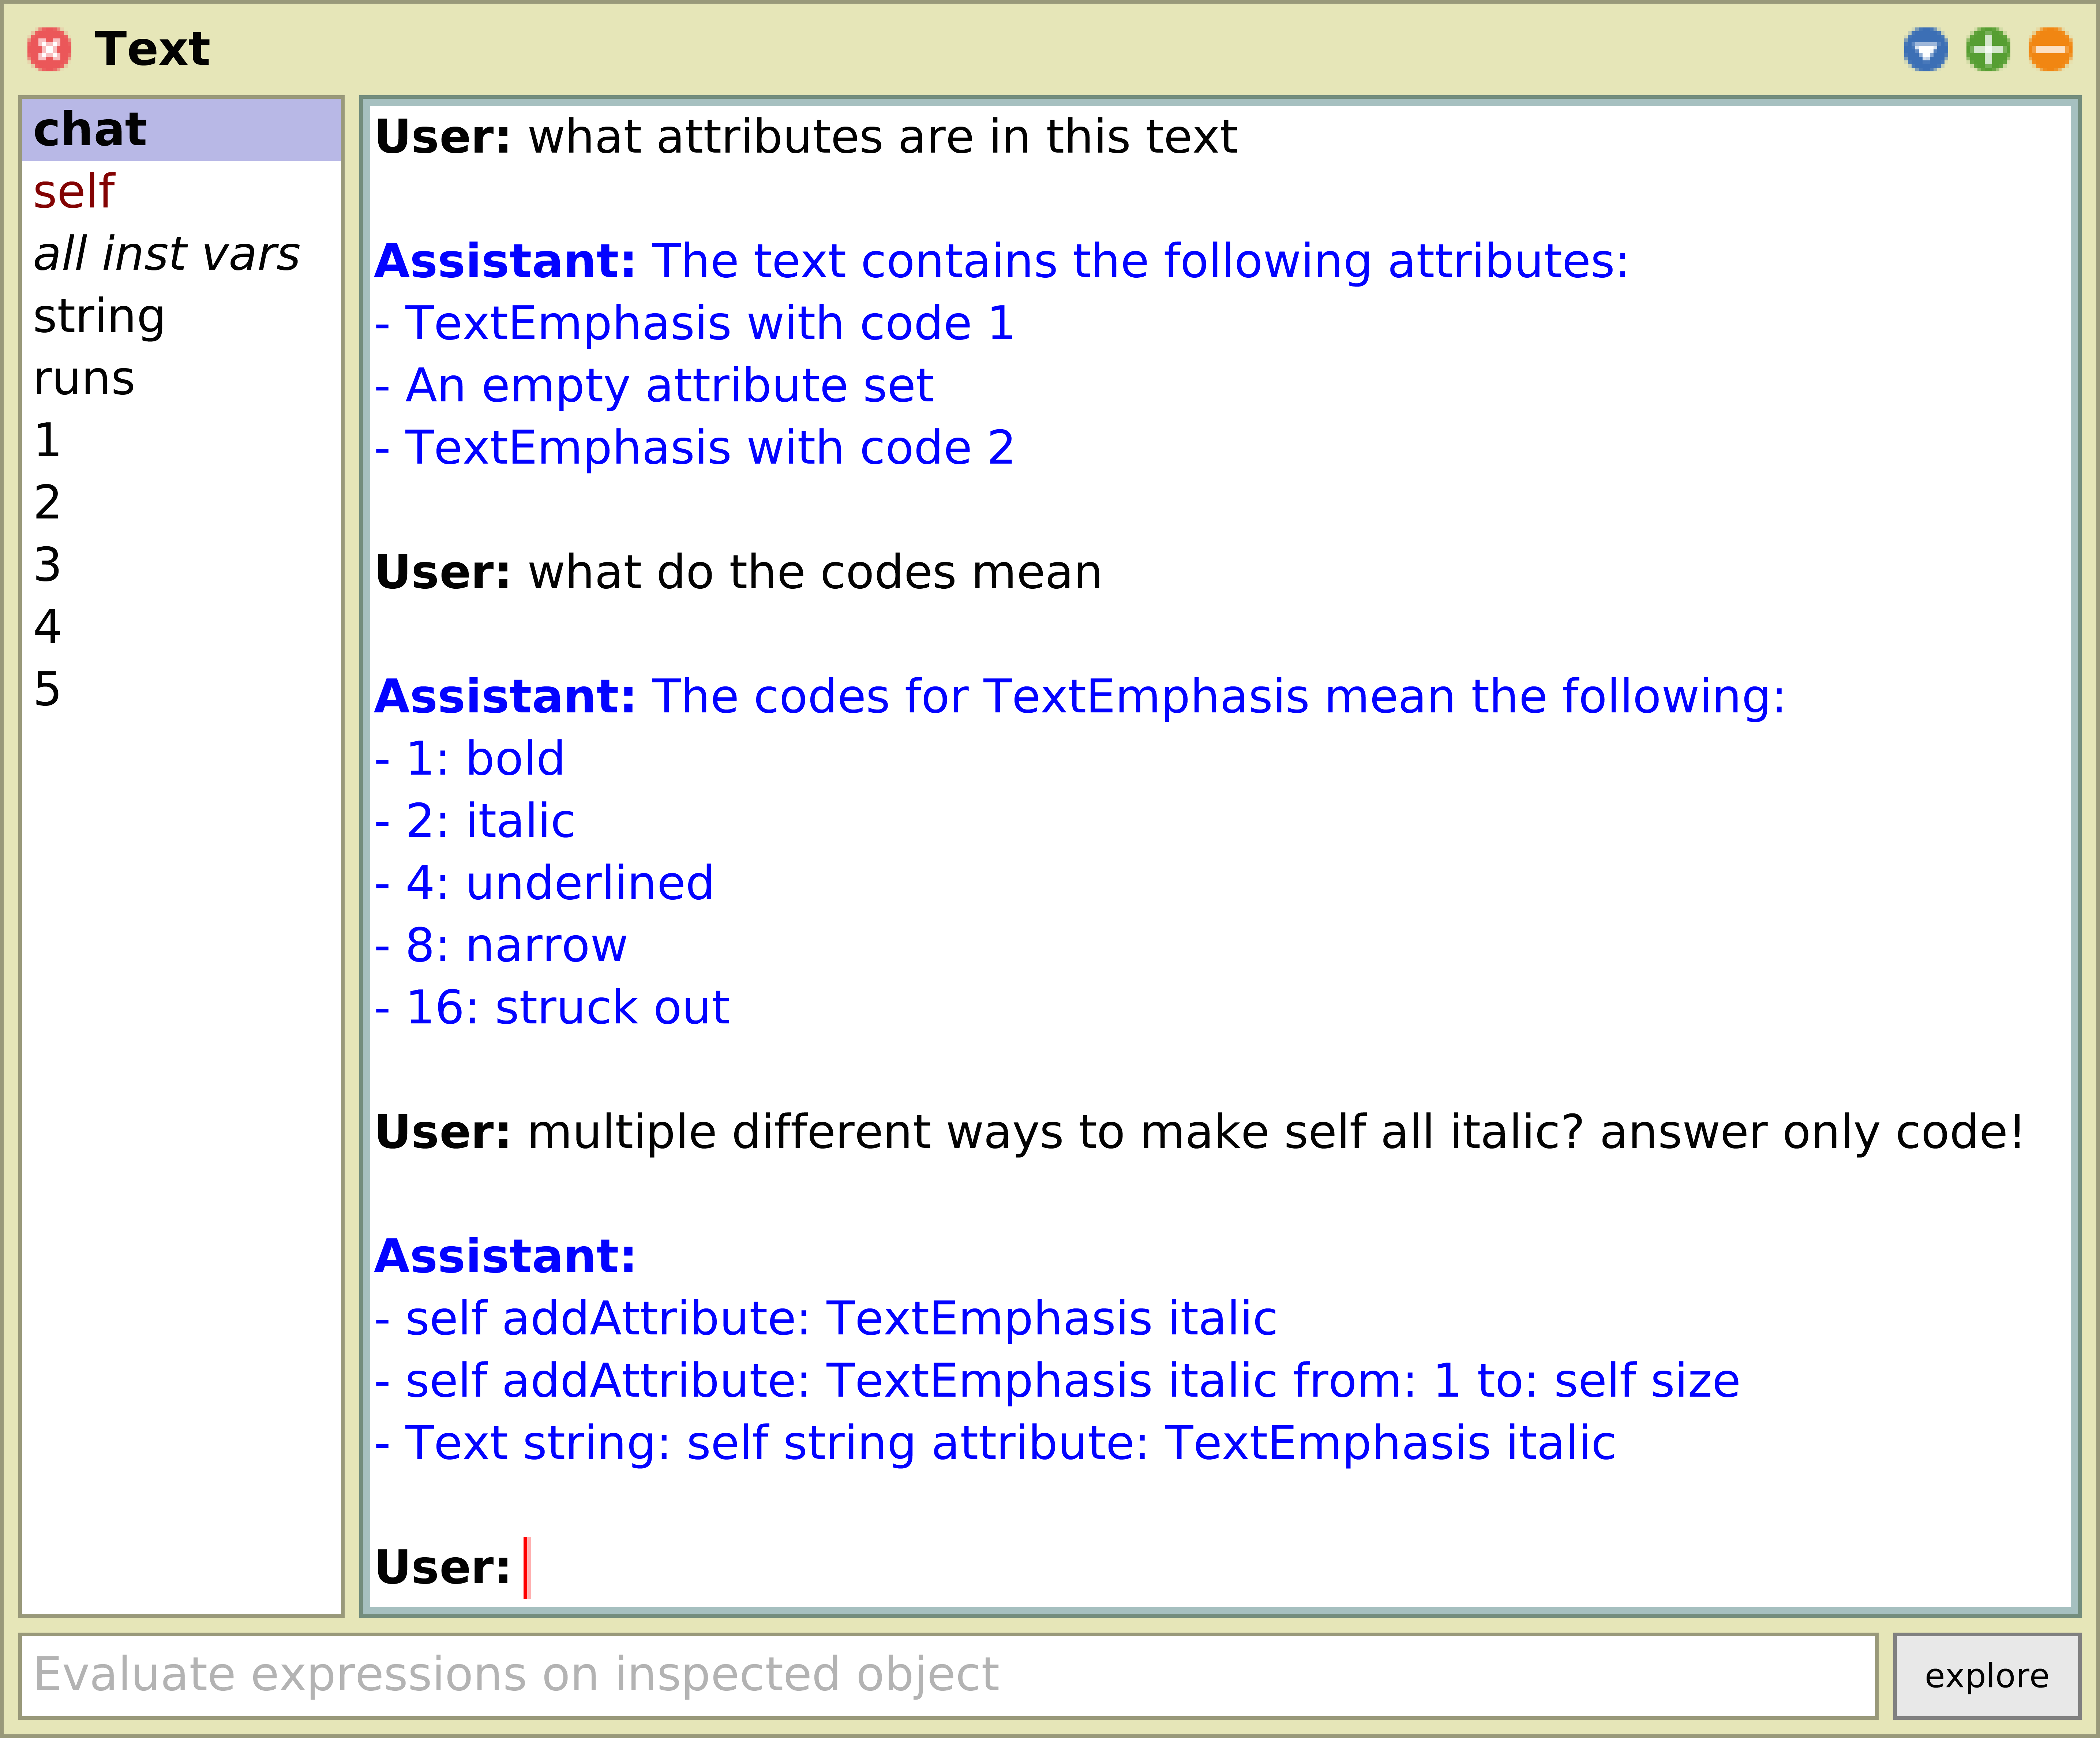
\includegraphics[width=0.9\textwidth]{chapters/08_application/02_conversation/text.png}
	\caption[Using the semantic conversation mode in an inspector to chat with a formatted \code{Text} object.]{
		Using the semantic conversation mode in an inspector to chat with a formatted \code{Text} object.
		Through the chat, the programmer can understand the attributes used for formatting and explore the available protocols for applying other formats to texts.
	}
	\label{fig:application/conversation/text}
\end{figure}

To start their exploration, the programmer discovers an existing \code{Text} object in the system that looks like this:

\begin{quote}
	\fbox{\textsf{\textbf{ABC}D\underline{E}}}\,%
	\footnote{Alternative description for accessibility: The first three letters are emphasized in bold, and the last letter is underlined.}
\end{quote}

To understand its design and behavior related to formatting, the programmer invokes an inspector on this text~(\cref{fig:application/conversation/text}).
First, they wonder what attributes are contained in the text.
As the internal structure of nested collections looks slightly overwhelming, they switch to the \emph{semantic conversation mode} of the inspector instead.
Here, they enter the following question:

\begin{quote}
	``What attributes are in this text?''
\end{quote}

In response, the exploratory programming agent automatically inspects the internal structure of the text, iterates over the nested collections, and finally lists both present attributes correctly in the chat: a ``TextEmphasis with code 1'' and a ``TextEmphasis with code 2''.
This points our programmer to the \code{TextEmphasis} class but also motivates them to learn more about its features and representation.
Thus, they type a follow-up question into the chat:

\begin{quote}
	``What do these codes mean?''
\end{quote}

Note that they can ask this within the context of the conversation---without needing to respecify the actual codes they are referring to or the class that defines them.
The agent processes this question by automatically browsing the documentation of the \code{TextEmphasis} class, locating the relevant information in its class comment, and printing the correct list of all emphasis codes into the chat.

Finally, the programmer wonders how they can add other emphases to the text, so they ask for several code examples to italicize the entire object.
In response, the agent automatically browses the protocols of the \code{Text} class, identifies and tests several possible messages, and provides three valid snippets to the programmer that would achieve the desired behavior.
The programmer can work with these snippets, adjust them with the help of the agent or by themselves, or integrate them into their own program.

\begin{figure}
	\centering
	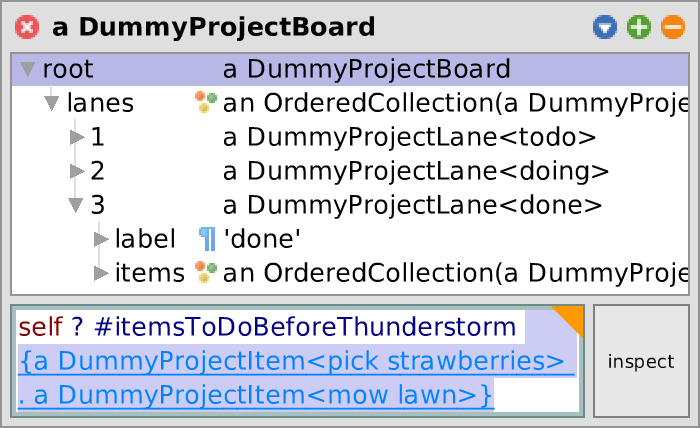
\includegraphics[width=0.6\textwidth]{chapters/08_application/02_conversation/project.png}
	\caption[Sending a semantic message to search and filter a small project management system for common-sense questions.]{
		Sending a semantic message to search and filter a small project management system for common-sense questions.
		The exploratory programming agent automatically explores the available protocols of the project management systems to retrieve items from the lanes of the project board and then filters them.
	}
	\label{fig:application/conversation/project}
\end{figure}

This scenario shows that the conversation mode in inspection tools can be used to answer a wide range of questions:
through functional questions, programmers can access, search, or summarize domain information.
Another example of this is filtering items in a task management system based on their content~(\cref{fig:application/conversation/project}).
Through epistemic questions, programmers can get familiar with domains, explore systems and interfaces, and prototype ideas as working applications.
In other settings, this could be used to study the different sorting protocols of collections, brainstorm and compare different options for formatting dates, or iteratively create visualizations.

In summary, programmers can use semantic conversations to ask semantic questions about objects, which the agent attempts to answer by extracting, analyzing, and synthesizing information.
Thus, programmers can maintain their workflow of exploring a domain from a conceptual perspective for a longer period of time without being overwhelmed or distracted by performing manual technical experiments.
